\documentclass[aps,pre,reprint,superscriptaddress,amsmath,amssymb]{revtex4-2}
\usepackage{graphicx}
\usepackage{bm}
\usepackage{hyperref}
\usepackage{booktabs}

% Every number in this file must come from a committed results/metrics.json.
% Numbers marked \TODO{} are pending a final clean-commit rerun (action plan R7).
\newcommand{\TODO}[1]{\textcolor{red}{[#1]}}
\usepackage{xcolor}

\begin{document}

\title{Discrete-exact energy accounting for FDTD simulations of time-modulated cavities:\\
separating pump work from numerical artifacts}

\author{Nielsen Castelo Damasceno Dantas}

\date{\today}

\begin{abstract}
Time-modulated electromagnetic media and cavities underpin parametric amplification,
temporal metamaterials and analogues of the dynamical Casimir effect. In such
systems the field energy is not conserved: the modulation performs work. Telling
that physical pump work apart from discretization error is essential, especially
when simulations drive automated optimization or are used to evaluate extraordinary
energy claims. We show that the Yee finite-difference time-domain (FDTD) scheme in
$D$-formulation, with time-varying permittivity, semi-implicit conduction, soft
sources and absorbing ports, satisfies an exact discrete energy balance. The
modulation contributes the closed-form pump work
$\tfrac12 D^nD^{n+1}(1/\varepsilon^{n+1}-1/\varepsilon^n)\Delta x$, and the full
ledger closes to floating-point round-off. Textbook energy estimators instead leave
residuals that converge at first or second order and are biased toward
\emph{apparent net generation}. They report gain at 92\% of the points of a
parametric resonance map, and even in a passive decaying cavity. An unconstrained
optimizer reading such a ledger ``discovers'' configurations that create 154\% of
the energy scale, all on the coarsest grids. The audited solver reproduces
Hill--Floquet theory, including the threshold $\delta_{\rm th}=2/Q$ and both Floquet
branches, and agrees at second order with an independent fourth-order
method-of-lines solver in a multimode case. A multimode stress test shows that
ledger closure is necessary but not sufficient. We release CavityLab, an
open-source library that makes this audit the default.
\end{abstract}

\maketitle

%=====================================================================
\section{Introduction}
%=====================================================================

Time-varying media have become a central topic in photonics~\cite{Galiffi2022}:
temporal interfaces, photonic time crystals and spacetime-modulated
metamaterials~\cite{Caloz2020}, and parametric and dynamical-Casimir-effect (DCE)
platforms~\cite{Wilson2011,Dodonov2020}. Their defining property is that the
electromagnetic energy is not conserved, because the agent that modulates the
medium does work on the field. The physics of that work is subtle. It depends on
which constitutive quantity is continuous at a temporal interface~\cite{Galiffi2025},
and on dispersion and pump realism~\cite{Hayran2022}. Lumped-circuit analyses book
it explicitly~\cite{Mirmoosa2019}.

Numerical studies of such systems routinely use FDTD with
$\varepsilon(x,t)$~\cite{Stewart2016,Taravati2024,Sarkar2022,Faccio2011}. In those
studies the energy budget is either not reported or is evaluated with continuum
formulas applied to the discrete fields. This is a verification gap. If the
bookkeeping is not consistent with the discretization, the residual of the energy
balance mixes three things: physical pump work, physical loss, and numerical error.
A residual of the wrong sign looks like energy appearing from nowhere.

The risk is not academic. Automated design loops and optimizers are known to
exploit simulator artifacts~\cite{Lehman2018}. Separately, claims of extracting
energy from the quantum vacuum have a long history~\cite{Forward1984,Cole1993},
and none has been reliably demonstrated~\cite{Moddel2019}. The static Casimir force
does not even require invoking the absolute vacuum energy~\cite{Jaffe2005}.
Evaluating such claims, or simply building trustworthy pipelines for time-modulated
photonics, requires an energy audit whose own error is known and negligible.

For the lossless Yee scheme a discrete energy is classical: it underlies
energy-method stability proofs~\cite{Joly2003,Chen2008,Bekmambetova2016}. We do not
claim it as new. Our contributions are:

\begin{enumerate}
\item The extension of that identity to the terms that matter in modulated cavities
  (time-varying permittivity, conduction, sources, ports), including a closed-form
  discrete pump-work term, so that the complete ledger closes to round-off.
\item A taxonomy of the errors of naive (continuum-formula) ledgers, with their
  convergence orders and their sign bias.
\item Verification against Hill--Floquet theory and an independent solver.
\item A demonstration that an optimizer exploits naive ledgers and that the audit
  rejects every such ``discovery''.
\end{enumerate}

%=====================================================================
\section{Discrete energy identity}
%=====================================================================

We consider the $E_z/H_y$ polarization on $[0,L]$ with perfect-electric-conductor
(PEC) walls. $D_i^n$ and $E_i^n$ live on the nodes $x_i=i\Delta x$ and
$H_{i+1/2}^{n+1/2}$ on the half nodes. The scheme is
\begin{align}
H^{n+1/2}_{i+1/2} &= H^{n-1/2}_{i+1/2} + \frac{\Delta t}{\mu\Delta x}\left(E^n_{i+1}-E^n_i\right),\\
D^{n+1}_i &= D^n_i + \frac{\Delta t}{\Delta x}\left(H^{n+1/2}_{i+1/2}-H^{n+1/2}_{i-1/2}\right)
 - \Delta t\,\sigma_i\bar E_i - \Delta t\,J_i^{n+1/2},\\
E^{n+1}_i &= D^{n+1}_i/\varepsilon_i^{n+1},\qquad \bar E_i=\tfrac12\left(E^n_i+E^{n+1}_i\right).
\end{align}
Define the discrete stored energy (per unit transverse area)
\begin{equation}
W^n = \frac{\Delta x}{2}\sum_i D^n_iE^n_i + \frac{\mu\Delta x}{2}\sum_j H^{n+1/2}_jH^{n-1/2}_j .
\end{equation}

Splitting $\tfrac12(D'E'-DE) = \tfrac12(D'-D)(E'+E) + \tfrac12(DE'-D'E)$ and summing
the Maxwell exchange terms by parts (they cancel with PEC walls) gives the exact
one-step balance
\begin{multline}
W^{n+1}-W^n = \Delta x\sum_i\Big[\tfrac12 D_i^nD_i^{n+1}\Big(\frac{1}{\varepsilon_i^{n+1}}-\frac{1}{\varepsilon_i^n}\Big)\\
-\Delta t\,\sigma_i\bar E_i^2-\Delta t\,J_i^{n+1/2}\bar E_i\Big].
\label{eq:balance}
\end{multline}

The first term is the work done by the modulation. Its continuum limit is
$-\tfrac12E^2\partial_t\varepsilon$, the work required to change $\varepsilon$ at
fixed $D$. The second term is the dissipation, booked as output in absorbing-port
regions. The third term is the source work. Equation~\eqref{eq:balance} holds for
any $\sigma\ge0$, any $\varepsilon(x,t)>0$ and any Courant number below the CFL
limit. With the sign convention
\begin{equation}
E_{\rm net} = E_{\rm out}+E_{\rm loss}+\Delta W - E_{\rm in},
\end{equation}
exact bookkeeping gives $E_{\rm net}=0$ up to round-off, which grows roughly like
$n_{\rm steps}\,\epsilon_{\rm mach}$.

%=====================================================================
\section{Naive ledgers}
%=====================================================================

Typical post-processing evaluates continuum expressions pointwise:

\begin{itemize}
\item stored energy $\tfrac12\varepsilon(E^n)^2+\tfrac12\mu(\bar H^n)^2$, with
  $\bar H^n$ the average of the two half steps;
\item left-point dissipation $\sigma\Delta t(E^n)^2$;
\item left-point source work $-\Delta tJE^n$;
\item left-point pump work $-\tfrac12(E^n)^2(\varepsilon^{n+1}-\varepsilon^n)$.
\end{itemize}

The first produces an oscillating $O((\omega\Delta t)^2)$ residual; the left-point
rules produce cumulative $O(\Delta t)$ residuals. Table~\ref{tab:naive} summarizes
the measured levels.

\begin{table}[t]
\caption{Exact vs naive ledgers, $N=400$ cells per cavity, $S=0.5$ (EXP-0003/0004).}
\label{tab:naive}
\begin{ruledtabular}
\begin{tabular}{lccc}
Scenario & exact & naive max & naive final \\
\hline
Closed, lossless & $4\times10^{-15}$ & $1.5\times10^{-4}$ & $-8.1\times10^{-5}$\\
Free decay, $Q=50$ & $6\times10^{-13}$ & $1.6\times10^{-4}$ & $\bm{+1.6\times10^{-4}}$\\
Driven, $Q=100$ & $1.9\times10^{-12}$ & $2.3\times10^{-5}$ & $-2.2\times10^{-5}$\\
Open port & $3.5\times10^{-15}$ & $2.7\times10^{-4}$ & $-4.0\times10^{-6}$\\
\end{tabular}
\end{ruledtabular}
\end{table}

%=====================================================================
\section{Verification in static cavities}
%=====================================================================

All runs use $L=0.1$~m, float64 and $S=c\Delta t/\Delta x=0.5$ unless stated
otherwise. $S=1$ is the dispersionless ``magic'' step in 1D and would hide
dispersion errors.

\paragraph{Modes and dispersion (EXP-0001).} Exact discrete eigenmodes oscillate at
the Yee dispersion frequency. The measured frequency agrees with it to
$2.7\times10^{-12}$, and the discrete energy drifts by $3\times10^{-15}$. The error
relative to $\omega_n=n\pi c/L$ follows $-(k\Delta x)^2(1-S^2)/24$.

\paragraph{Convergence (EXP-0002).} A Gaussian pulse is compared with the exact
d'Alembert/image solution. The observed orders are 1.998, 1.999 and 2.001 for
$S=0.25$, 0.5 and 0.9. At $S=1$ the error is at round-off.

\paragraph{Ledgers (EXP-0003).} Table~\ref{tab:naive} and Fig.~\ref{fig:static}
cover four scenarios. The exact ledger closes to between $4\times10^{-15}$ and
$1.9\times10^{-12}$; the larger value corresponds to $4.8\times10^5$ steps. The $Q$
factor measured from the free decay is 50.001, against an analytic value of 50. The
naive residuals vanish under refinement:
\begin{itemize}
\item the time-averaged energy converges at order 2.1;
\item the left-point source and dissipation rules converge at order 0.9;
\item the open-port case converges at order 1.2.
\end{itemize}
Notably, the naive ledger of a \emph{passive} decaying cavity reports net
generation of $+1.6\times10^{-4}$ of the energy scale.

\begin{figure}[t]
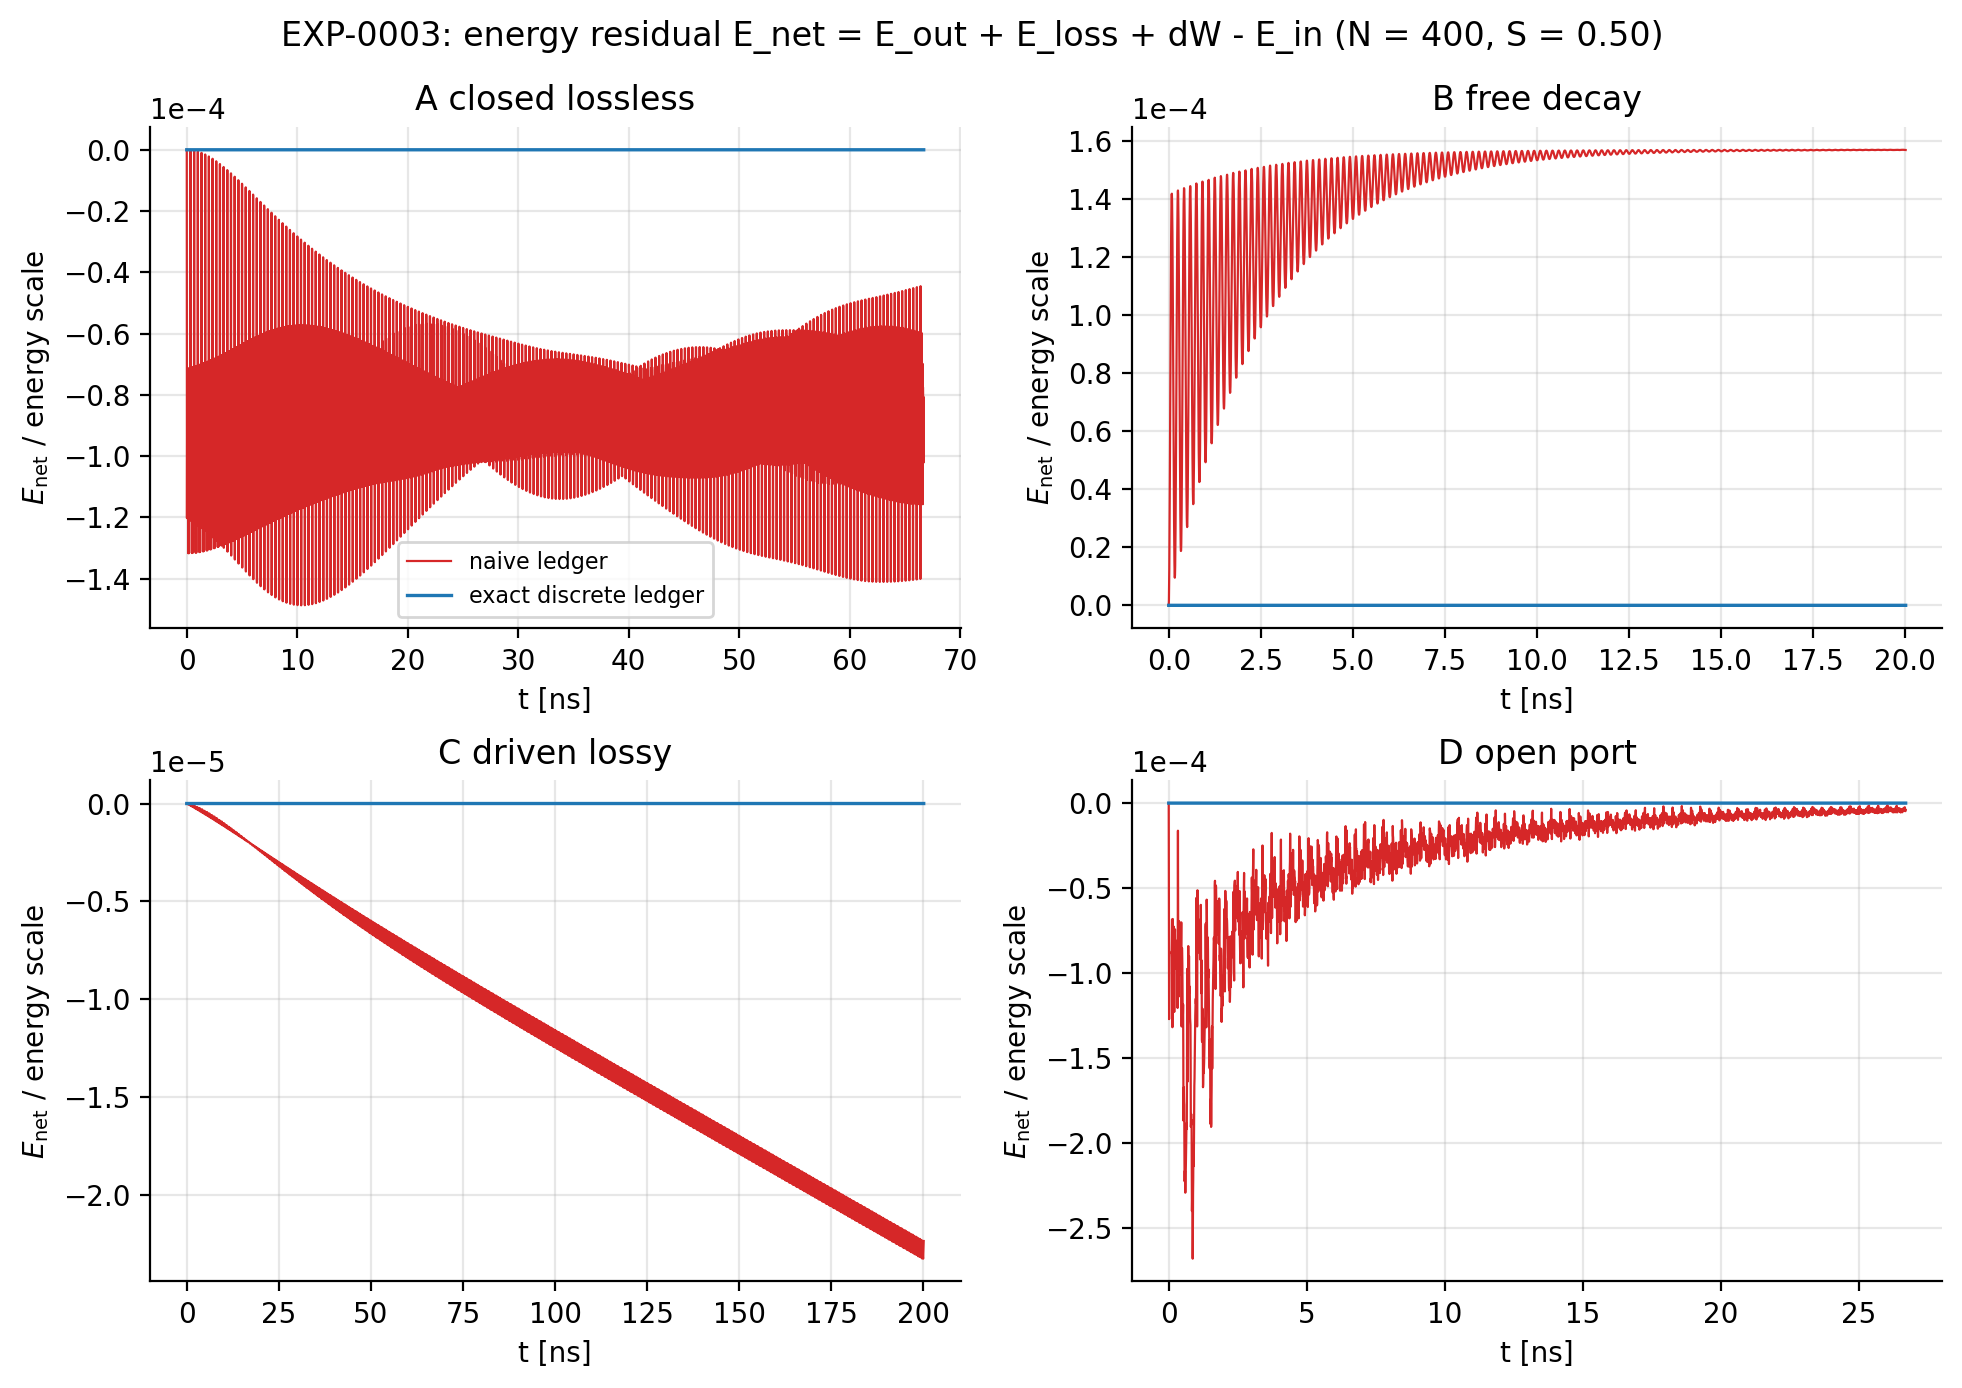
\includegraphics[width=\columnwidth]{../../experiments/EXP-0003_static_energy_balance/figures/exp0003_energy_residuals.png}
\caption{$E_{\rm net}$ normalized by the energy scale for the exact discrete ledger
(blue) and a naive ledger (red) in four static scenarios (EXP-0003).}
\label{fig:static}
\end{figure}

%=====================================================================
\section{Parametrically modulated cavities}
%=====================================================================

\paragraph{Hill reduction.} For $\varepsilon(t)=\varepsilon_s f(t)$ with
$f=1+\delta\sin(\Omega t+\phi)$ filling the cavity, every mode decouples, both in
the continuum and on the grid. In dimensionless form ($\tau=\omega_mt$,
$p=d/\varepsilon_s$, $q=\eta_sh$) the mode equations are
\begin{equation}
\dot p=-q-\frac{p}{Qf},\qquad \dot q=\frac{p}{f},\qquad w=\frac{p^2}{f}+q^2 .
\end{equation}
Near $\Omega=2\omega_m$ the amplitude Floquet exponents are
$\pm\delta/4-1/(2Q)$, so the threshold is $\delta_{\rm th}=2/Q$.

\paragraph{FDTD monodromy.} We measure the $2\times2$ monodromy matrix directly from
two FDTD runs started in the two field quadratures. This matters: a start in a
single quadrature with $\phi=0$ lies \emph{exactly} on the decaying branch
($-\gamma-\delta\omega/2$). Naive growth-rate fits can then disagree with theory by
orders of magnitude, although nothing is wrong with the solver (EXP-0004).

With $Q=200$:
\begin{itemize}
\item the Floquet rates from FDTD match Hill theory to within $0.1\%$ of $\omega/Q$
  for $\delta/\delta_{\rm th}=0.5$, 1, 2 and 4;
\item the stored energy converges to the ODE at order 2.00;
\item the exact ledger closes to below $3\times10^{-14}$, whereas the naive ledger
  is at $10^{-4}$ to $10^{-3}$ and its sign changes with resolution.
\end{itemize}

\paragraph{Resonance maps (EXP-0005).} Over the $(\nu=\Omega/\omega_1,\delta)$ plane:
\begin{itemize}
\item stability classification from the FDTD monodromy agrees with theory at
  \TODO{100\%} of points;
\item the exact ledger closes to \TODO{$<2\times10^{-13}$} everywhere;
\item the naive ledger reports apparent gain at \TODO{92\%} of points, up to
  \TODO{26\%} of the energy scale;
\item at the worst point that gain halves with every doubling of resolution
  (order \TODO{1.02}).
\end{itemize}
The left-point pump-work rule is therefore positively biased.

%=====================================================================
\section{Multimode cases}
%=====================================================================

\paragraph{Equidistant spectrum (stress test).} In an empty cavity
$\omega_k=k\omega_1$. Under localized modulation at $2\omega_1$ the resonant
cascade feeds ever higher modes, and the continuum problem has no resolvable
limit. The stored energy after 20 periods \emph{increases} with resolution (from
117 at $N=200$ to 247 at $N=1600$). The exact ledger still closes to
$4\times10^{-15}$, while the naive ledger reports gains of $+0.35\%$ and $+0.13\%$
of the pump input at $N=100$ and 200. Ledger closure is necessary, not sufficient.

\paragraph{Non-equidistant spectrum (converged).} A smooth dielectric step makes
$\omega_k/\omega_1=1, 2.07, 3.01, 4.11,\dots$, and the problem converges. We compare
against an independent method-of-lines solver: fourth-order staggered differences
with PEC images and adaptive DOP853 time integration. That solver is verified at
order 4.00 and is self-converged to $2\times10^{-7}$.
\begin{itemize}
\item The FDTD stored energy converges to the reference at order 1.995, from an
  error of $2.1\times10^{-2}$ at $N=100$ to $8.1\times10^{-5}$ at $N=1600$
  (EXP-0004c).
\end{itemize}

%=====================================================================
\section{Artifacts under optimization}
%=====================================================================

We let a seeded random search maximize the naive $E_{\rm net}$ over $\nu$, $\delta$,
$N$ and $S$, as a careless automated pipeline might (EXP-0005b, Fig.~\ref{fig:opt}).
\begin{itemize}
\item The naive objective is positive in $92.7\%$ of 300 trials.
\item The best ``design'' creates $154\%$ of the energy scale.
\item The optimizer gravitates to the coarsest grids ($N=24$--32), exploiting
  resolution rather than physics.
\end{itemize}
Two cheap checks reject all five top candidates: the exact ledger
($|E_{\rm net}|/{\rm scale}\le1.5\times10^{-14}$ across all trials) and refinement,
under which the naive gain halves with each doubling of $N$.

\begin{figure}[t]
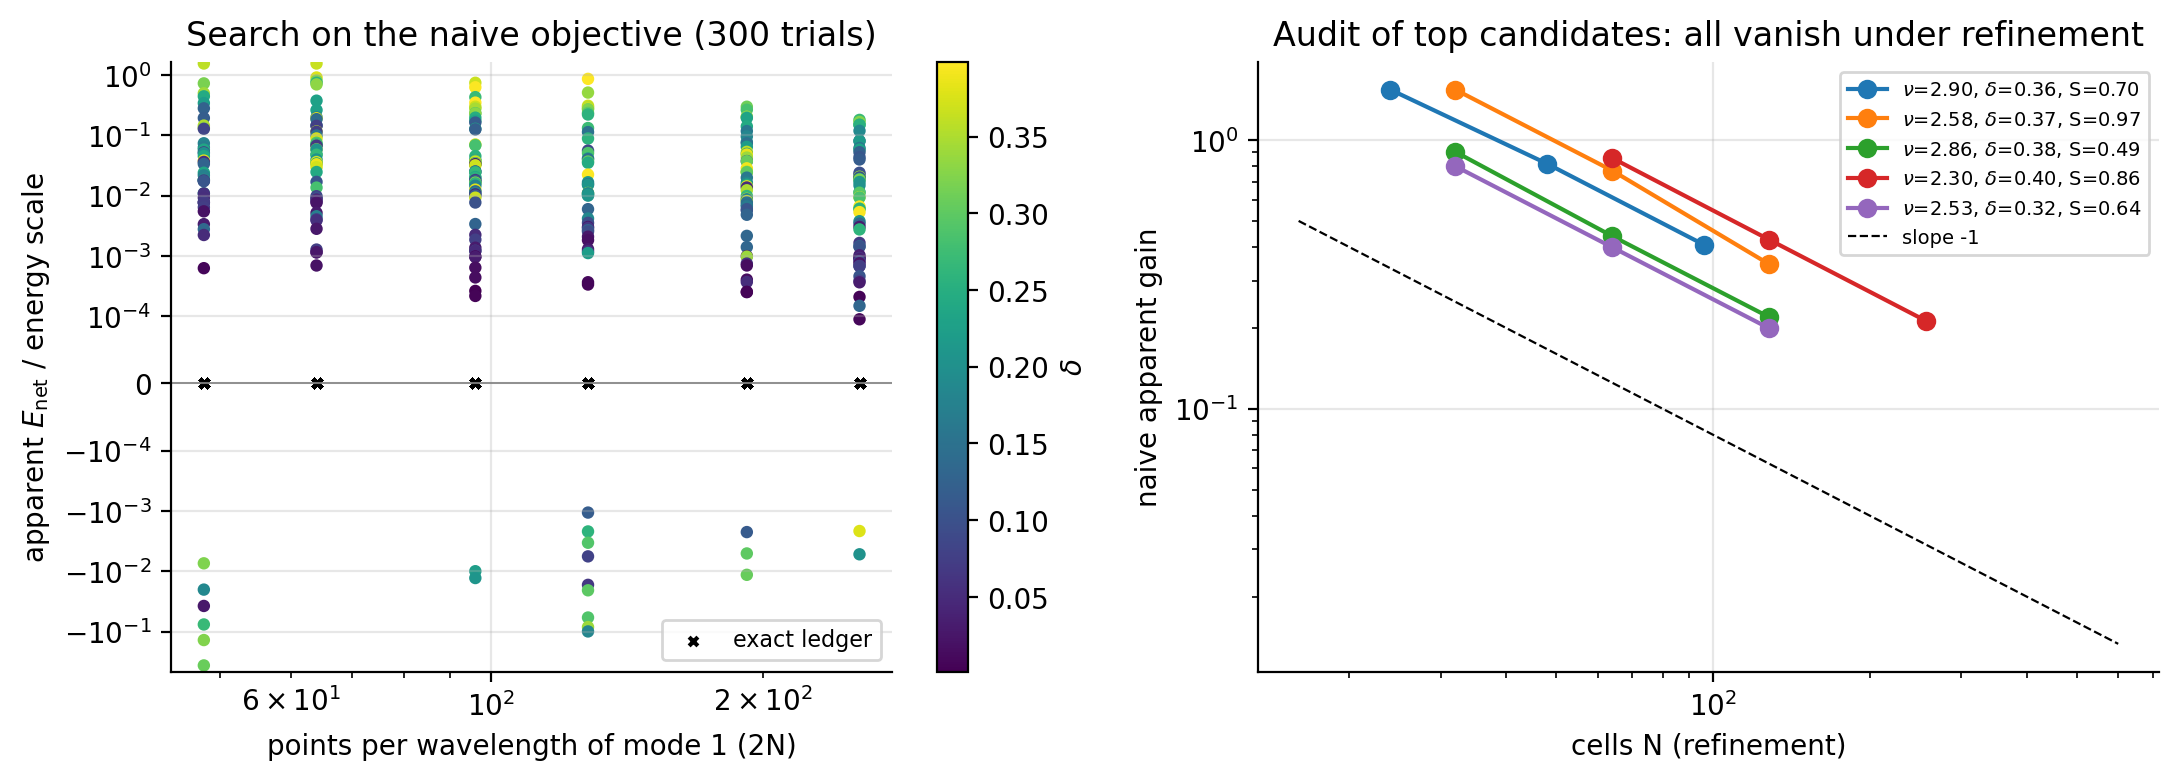
\includegraphics[width=\columnwidth]{../../experiments/EXP-0005b_optimizer_exploit/figures/exp0005b_optimizer_exploit.png}
\caption{Left: naive objective (colored by $\delta$) and exact ledger (crosses) for
300 random trials. Right: refinement of the five best naive candidates.}
\label{fig:opt}
\end{figure}

%=====================================================================
\section{Discussion}
%=====================================================================

The discrete-exact ledger turns energy conservation from a qualitative sanity check
into a quantitative test with a round-off floor (Sec.~II). Any residual above that
floor is a bug, and any apparent net generation in a naive ledger is a
discretization artifact with a known order.

Two caveats emerged.
\begin{enumerate}
\item A closed ledger does not certify accuracy. The equidistant multimode case
  closes to round-off while being unresolved. Convergence studies and an
  independent reference remain indispensable.
\item Comparisons with Floquet theory must use the full monodromy, because special
  initial conditions can select a single branch.
\end{enumerate}

For optimization and automated discovery we recommend three rules:
\begin{enumerate}
\item use the exact ledger in the objective;
\item never let numerical parameters be design variables;
\item re-audit candidates at higher resolution before reporting them.
\end{enumerate}

The construction extends to 2D/3D Yee grids, to PML regions (as port terms) and to
dispersive media through auxiliary-field energies; these extensions are left for
future work.

\paragraph*{Code and data availability.} CavityLab (MIT license) contains the solver,
the audit and one script per figure, with manifests recording git commit,
environment and configuration hash. \TODO{Zenodo DOI.}

\bibliography{refs}

\end{document}
